
% ----------------------------------------------------------------------
%  Set the document class
% ----------------------------------------------------------------------
\documentclass[11pt,a4paper,twoside]{article}

% ----------------------------------------------------------------------
% Define external packages, language, margins, fonts and new commands
% ----------------------------------------------------------------------
%\input{preamble} 
\usepackage[utf8]{inputenc}   % <<<<< Linux
\usepackage[english]{babel} % <<<<< English
\usepackage{notoccite}
\usepackage[skip=0.5\baselineskip]{caption}
\hyphenation{GTKWave}
\usepackage{listings}
\usepackage[all]{nowidow}
\usepackage{amsmath}
\usepackage{placeins}

%blind text
%\usepackage{lipsum}

\usepackage{graphicx}
\graphicspath{ {./} {../../figlib/} }
\def\FontLn{% 16 pt normal
  \usefont{T1}{phv}{m}{n}\fontsize{16pt}{16pt}\selectfont}
\def\FontLb{% 16 pt bold
  \usefont{T1}{phv}{b}{n}\fontsize{16pt}{16pt}\selectfont}
\def\FontMn{% 14 pt normal
  \usefont{T1}{phv}{m}{n}\fontsize{14pt}{14pt}\selectfont}
\def\FontMb{% 14 pt bold
  \usefont{T1}{phv}{b}{n}\fontsize{14pt}{14pt}\selectfont}
\def\FontSn{% 12 pt normal
  \usefont{T1}{phv}{m}{n}\fontsize{12pt}{12pt}\selectfont}

% Use Arial font as default
%
\renewcommand{\rmdefault}{phv}
\renewcommand{\sfdefault}{phv}
\usepackage{geometry}	
\geometry{verbose,tmargin=2.5cm,bmargin=2.5cm,lmargin=2.5cm,rmargin=2.5cm}
\usepackage{mathtools}	
%\usepackage{setspace}
%\renewcommand{\baselinestretch}{1.5}

\usepackage[pdftex]{hyperref} % enhance documents that are to be
                              % output as HTML and PDF
\hypersetup{colorlinks,       % color text of links and anchors,
                              % eliminates borders around links
%            linkcolor=red,    % color for normal internal links
            linkcolor=black,  % color for normal internal links
            anchorcolor=black,% color for anchor text
%            citecolor=green,  % color for bibliographical citations
            citecolor=black,  % color for bibliographical citations
%            filecolor=magenta,% color for URLs which open local files
            filecolor=black,  % color for URLs which open local files
%            menucolor=red,    % color for Acrobat menu items
            menucolor=black,  % color for Acrobat menu items
%            pagecolor=red,    % color for links to other pages
            pagecolor=black,  % color for links to other pages
%            urlcolor=cyan,    % color for linked URLs
            urlcolor=black,   % color for linked URLs
	          bookmarks=true,         % create PDF bookmarks
	          bookmarksopen=false,    % don't expand bookmarks
	          bookmarksnumbered=true, % number bookmarks
	          pdftitle={report},
            pdfauthor={Andre C. Marta},
%            pdfsubject={Thesis Title},
%            pdfkeywords={Thesis Keywords},
            pdfstartview=FitV,
            pdfdisplaydoctitle=true}

\usepackage[numbers,sort&compress]{natbib} % <<<<< References in numbered list [1],[2],...
\usepackage{subcaption} 
\usepackage{mdframed}
\usepackage{float}
%%%%%%%%%%%%%%%%%%%%%%%%%%%%%%%%%%%%%%%%%%%%%%%%%%%%%%%%%%%%%%%%%%%%%%%%
%     Begin Document                                                   %
%%%%%%%%%%%%%%%%%%%%%%%%%%%%%%%%%%%%%%%%%%%%%%%%%%%%%%%%%%%%%%%%%%%%%%%%


\begin{document}

% Set plain page style (no headers, footer with centered page number)
\pagestyle{plain}

% Set roman numbering (i,ii,...) before the start of chapters
%\pagenumbering{roman}

% ----------------------------------------------------------------------
%  Cover page
% ----------------------------------------------------------------------
\thispagestyle {empty}


\includegraphics[bb=9.5cm 11cm 0cm 0cm,scale=0.29]{IST_A_CMYK_POS}

\begin{center}

\vspace{1.0cm}

% Title, author and degree
\vspace{1cm}
{\FontLb Circuit Theory and Electronics Fundamentals} \\ % <<<<< EDIT TITLE
\vspace{0.5cm}
{\FontSn Técnico, University of Lisbon} \\ % <<<<< EDIT COURSE
\vspace{0.5cm}
{\FontSn First laboratoy report} \\
\vspace{0.5cm}
{\FontSn Pedro Vilas, nº8631} \\
{\FontSn José Machado, nº95812} \\
{\FontSn Pedro Tomé, nº93151} \\
{\FontSn Group 68} \\


{\FontSn March 22, 2021} \\
\end{center}




% ----------------------------------------------------------------------
% Dedication page (optional)
% ----------------------------------------------------------------------
%\input{dedication} 
%\cleardoublepage

% ----------------------------------------------------------------------
%  Acknowledgments (optional)
% ----------------------------------------------------------------------
%\input{acknowledgements}
%\cleardoublepage

% ----------------------------------------------------------------------
%  Abstract (both in English and Portuguese)
% ----------------------------------------------------------------------
%\input{resumo} 
%\cleardoublepage

%\input{abstract} 

% ----------------------------------------------------------------------
%  Table of contents, list of tables, list of figures and nomenclature
% ----------------------------------------------------------------------

% Table of contents
\pagebreak
\tableofcontents
\vspace{15cm}
\pagebreak
% List of tables
%\addcontentsline{toc}{section}{\listtablename}
%\listoftables
%\cleardoublepage 

% List of figures
%\addcontentsline{toc}{section}{\listfigurename}
%\listoffigures
%\cleardoublepage 

% Set arabic numbering (1,2,...) after preface
%
%\setcounter{page}{1}
%\pagenumbering{arabic}

% ----------------------------------------------------------------------
%  Body
% ----------------------------------------------------------------------
\pagebreak
\section{Introduction}
\label{sec:introduction}


\par The objective of this laboratory assignment was to create an audio amplifier circuit. The audio amplifier would recieve an audio input of 10mV (maximum) that would be connected to an 8 Ohm speaker. The source would have an 100 Ohm impedance and the circuit would be supplied with 12 volts by a DC source (Vcc).
\par A good voltage amplifier has to have an high gain $(A_{V})$, a low output impedance $(Z_{o})$ and a high input impedance $(Z_{i})$. So as to meet this criteria the audio amplifier circuit would have two stages: the gain stage and the output stage. This seemed to be the best way to combine the good and not so good properties of each of the amplifier circuits studied in class.\par
 In the gain stage was used a common emitter amplifier with degeneration because it allows us to have a high $Z_{i}$ and a high gain $A_{V}$. Unfortunately the output signal will be degraded because it has a high $Z_{o}$ as well. This problem is to be fixed in the next stage. In this stage an NPN transistor was used.\par
 In the output stage a commom collector amplifier was used in order to maintain the high gain $A_{V}$ from the previous stage whilst having a low $Z_{o}$. This stage is able to maintain the high gain due to the fact that its high input impedance connects to the lower output impedance (but still an high one) of the previous stage and the gain in this section is $\approx 1$. In this stage a PNP transistor was used.
\par   
To determine the quality of the audio amplifier when compared to others, was created a merit classification system. The following equation is the one that gives us the merit of the circuit: 
\begin {equation}
	 MERIT = \frac{Voltage Gain*Bandwidth}{Cost*Lower Cut Off Frequency}   	
	\label{eq:i1}
\end{equation}

and the cost of the components are the following: cost of resistors = 1 monetary unit (MU) per kOhm, cost of capacitors = 1 MU/uF
and cost of transistors = 0.1 MU per diode. 

The general layout of the circuit that was implemented can be seen in \textbf{Figure~\ref{fig:circuit_t4}}
\par
\begin{figure}[h] \centering
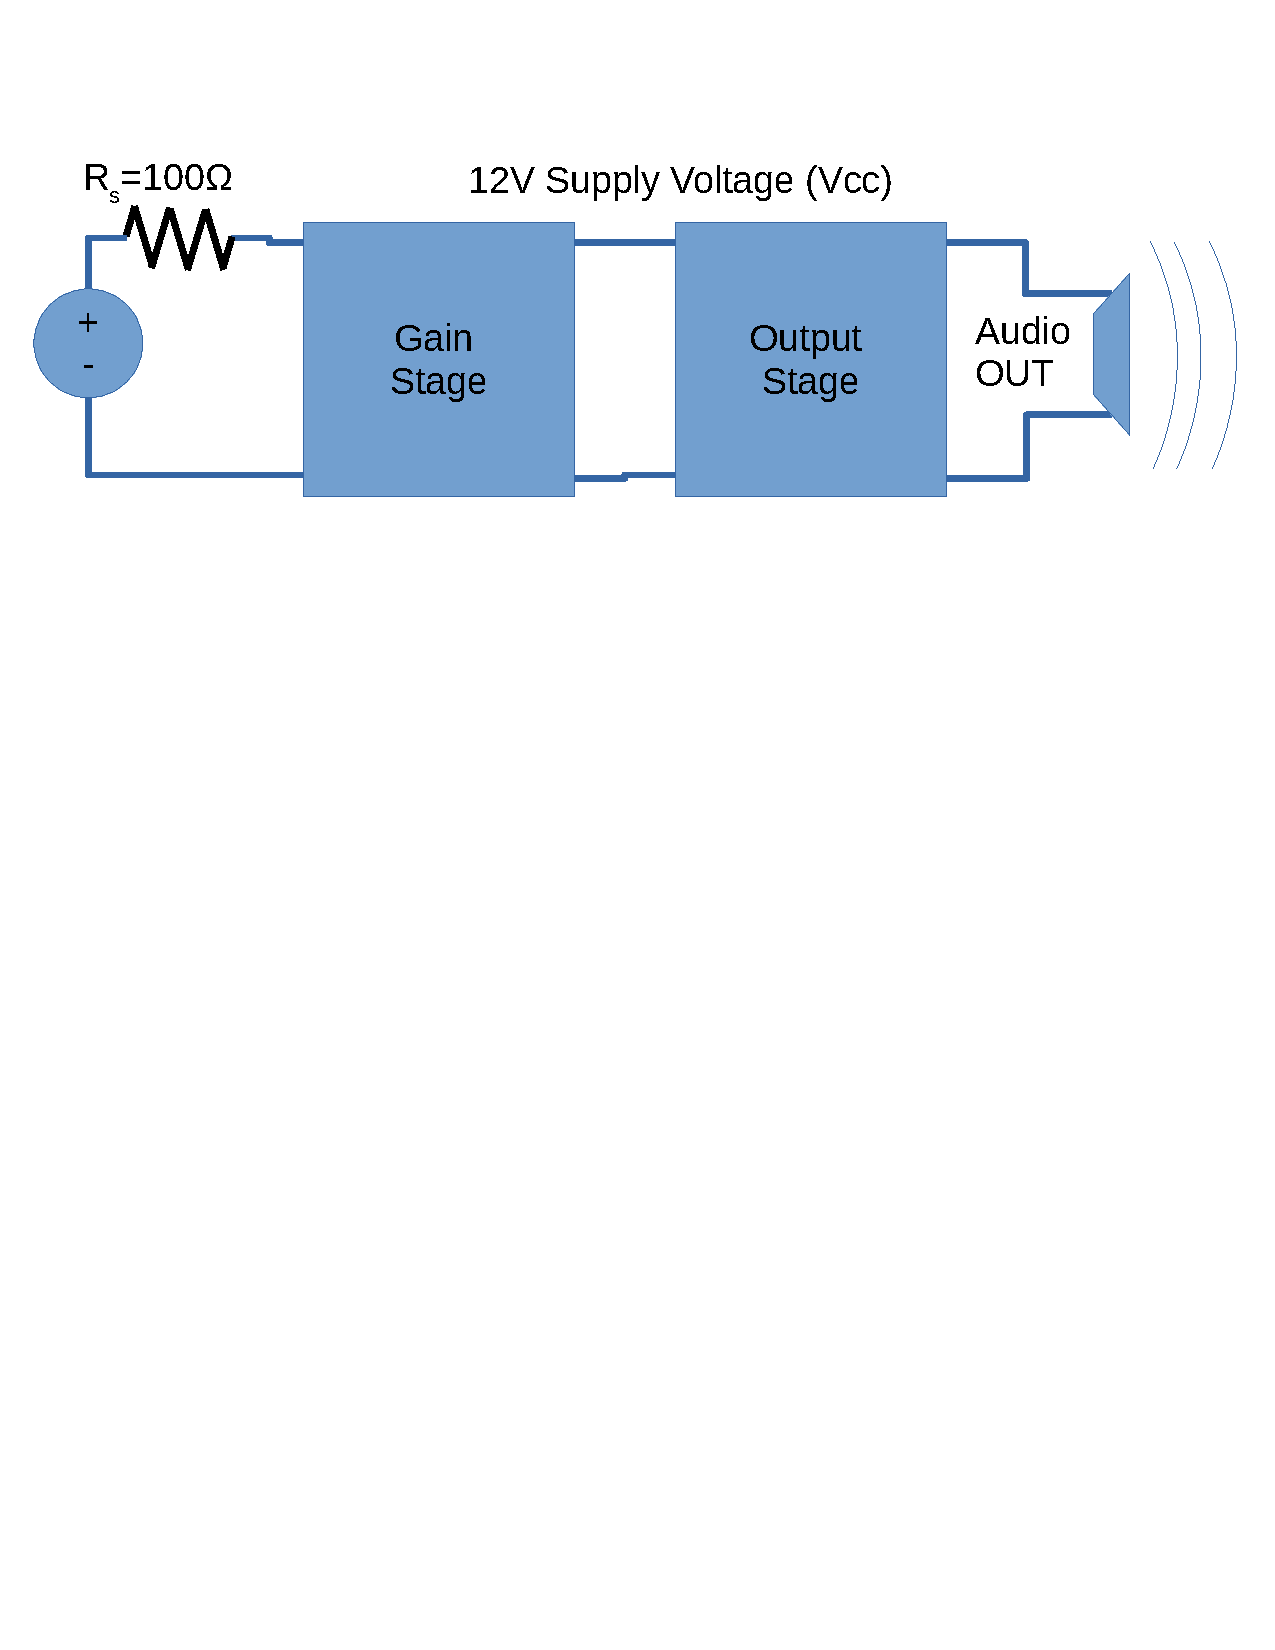
\includegraphics[width=0.6\linewidth]{circuit_t4.pdf}
\vspace{-6cm}
\caption{Circuit in study}
\label{fig:circuit_t4}
\end{figure}


In Section~\ref{sec:analysis}, we present a theoretical analysis of the circuit. Here the circuit is analised using the suitable OP (so as to make sure that the transistors are in the Forward Active Region) and incremental theoretical models studied in the class, in order to predict for each of the stages the gain and the input and output impedances.
In Section~\ref{sec:simulation}, the circuit is analysed by
simulation using the program Ngspice. In Ngspice the Philips BJT'S model BC557A (PNP) and BC547A (NPN) for the transistors were used. The input and output impedances, the lower and upper 3dB cut off frequencies, as well as the gain, were computed by simulation. The conclusions of this study are outlined in
Section~\ref{sec:conclusion}, where the theoretical results obtained in
Section~\ref{sec:analysis} are compared to the simulation results obtained in
Section~\ref{sec:simulation}.





\pagebreak


\pagebreak
\section{Análise Teórica}
\label{sec:analise_teorica}
Análise do circuito utilizando 2 processos teóricos: método das malhas e método do nós.
\subsection{Método das Malhas} 

Foram criadas 4 variáveis para a aplicação do método das malhas, a correntes das malhas. Esta variáveis estão identificadas pelas letras IA, IB,IC e ID, na figura apresentada abaixo, onde também podem ser observados os sentidos utilizados. Sabendo os valores destas correntes e aplicando a lei de Ohm, são calculados os valores das correntes em cada um dos componentes e as tensões nos nós. Para determinar as 4 correntes das malhas, foram utilizadas as equações apresentadas abaixo, que foram resolvidas com o auxílio do Octave. 

\begin {equation}
	R_1I_A + R_3(I_A+I_B) + R_4(I_A+I_C) = V_a
	\label{eq:malha1}
\end{equation}

\begin {equation}
	R_6I_A + R_7I_C + R_4(I_C+I_A) = K_cI_C
	\label{eq:malha2}
\end{equation}

\begin {equation}
	I_B = K_bR_3(I_A+I_B)
	\label{eq:malha3}
\end{equation}

\begin {equation}
	I_D = I_d
	\label{eq:malha4}
\end{equation}


\subsection{Método dos Nós} 

Na aplicação do método dos nós foram considerados 9 nós, ou seja foi adicionada uma fonte de corrente fictícia o nó 7 e a resistência 6, criando assim mais um nó. Isto, porque na simulação feita no Ngspice era necessário definir a corrente sobre a qual a fonte de tensão Vc depende. Para haver uma coerência entre as 2 análises, manteve-se esta fonte fictícia. Obtêm-se então 9 equações, 5 diretamente obtidas aplicando a Lei de Kirchoff para as correntes (KCL) em cada um dos nós não ligados a fontes de corrente, 2 obtidas fazendo a diferença potencial entre os terminais das fontes de tensão e, por fim, 2 definindo a voltagem no nó 0 como nula e igualando as voltagens V8 e V7. As equações são as seguintes:\par


\begin {equation}
	V_0 = 0
	\label{eq1}
\end{equation}
\begin {equation}
	V_8 = V_7
	\label{eqn}
\end{equation}
\begin {equation}
	\frac{V_2-V_4}{R_3} + \frac{V_2-V_3}{R_2} + \frac{V_2-V_1}{R_1} = 0
	\label{eq4}
\end{equation}
\begin {equation}
	\frac{V_1-V_2}{R_1} + \frac{V_0 - V_8}{R_6} + \frac{V_0 - V_4}{R_4} = 0
	\label{eq3}
\end{equation}
\begin {equation}
	\frac{V_5-V_4}{R_5} + K_b(V_2-V_4) = I_d
	\label{eq6}
\end{equation}
\begin {equation}
	\frac{V_7-V_6}{R_7} + \frac{V_7 - V_0}{R_6} = 0
	\label{eq7}
\end{equation}
\begin {equation}
	\frac{V_3-V_2}{R_2} = K_b(V_2-V_4) 
	\label{eq5}
\end{equation}
\begin {equation}
	V_1 - V_0 = V_a
	\label{eq8}
\end{equation}
\begin {equation}
	V_4 - V_6 = K_c \frac{V_0 - V_7}{R_6}
	\label{eq9}
\end{equation}

Os valores obtidos para as correntes em cada um dos componentes e para as voltagens em cada um dos nós estão representados na seguinte tabela:
 \pagebreak 
\begin{table}[h]
  \centering
  \begin{tabular}{|l|r|r|}
    \hline    
    {\bf Nome} & {\bf Método das Malhas} & {\bf Métodos dos Nós}\\ \hline
    \input{final_table}
  \end{tabular}
  \caption{As variáveis que representam correntes estão precedidadas pelo simbolo @ e expressas em miliampere (mA); As restantes variáveis representam tensões e estão expressas em Volt (V)}
  \label{tab:valores_teoricos}
\end{table}

Pode verificar-se resultados exatamente iguais entre os 2 métodos, tal como esperado.



\pagebreak
\section{Análise Ngspice}
\label{sec:simulacao}
Análise do circuito utilizando o programa Ngspice.
\subsection{Análise do Ponto de Operação}
\textbf Como mencionado na secção anterior, teve de ser criada uma fonte de tensão fictícia entre o nó 7 e a resistência 6 de valor nulo. A razão já foi mencionada anteriormente e deve-se apenas ao funcionamento do programa. Na tabela representada abaixo, podem ser observados os resultados obtidos na simulação.

\begin{table}[h]
  \centering
  \begin{tabular}{|l|r|}
    \hline    
    {\bf Nome} & {\bf Valores (mA or V)} \\ \hline
    \input{op_tab}
  \end{tabular}
  \caption{Ponto de operação. As variáveis que representam correntes estão precedidadas pelo simbolo @ e expressas em miliampere (mA); As restantes variáveis representam tensões e estão expressas em Volt (V)}
  \label{tab:op}
\end{table}

Pode ser observado que os valores obtidos coincidem com total precisão com os valores obtidos utilizando os métodos teóricos.

\pagebreak
\section{Conclusão}
\label{sec:conclusao}

O objetivo deste laboratório foi cumprido com sucesso. Os resultados obtidos utilizando os diferentes métodos teóricos e a simulação no programa Ngspice coincidiram com precisão total, o que era esperado no circuito analisado. Isto porque o mesmo é composto apenas por componentes lineares e, como tal, os resultados não devem sofrer alterações dependendo do método utilizado, tal como mencionado nas aulas. \par
Foi, portanto, um laboratório bastante útil para aplicar os conhecimentos teóricos obtidos nas aulas e perceber um pouco melhor o funcionamento deste tipo de circuitos. Para além disso, o laboratório foi também proveitoso para uma introdução às ferramentas utilizadas. Esta nova realidade obriga a uma adaptação constante e ferramentas como o Github, Ngspice e Latex podem ser bastante úteis para uma melhor iteração à distância. Foi também necessária uma integração com o sistema operativo Linux e os respetivos ficheiros Make, o que não foi propriamente fácil, mas que veio acrescentar conhecimento que poderá vir a ser útil no futuro. 


%\cleardoublepage

% ----------------------------------------------------------------------
%  Bibliography
% ----------------------------------------------------------------------
%\addcontentsline{toc}{section}{\bibname}
%\bibliographystyle{abbrvunsrtnat} % <<<<< SELECT IF USING REFERENCES BY NUMBER (CITATION ORDER)
%\bibliography{../../../BIBfile.bib}

% ----------------------------------------------------------------------
\end{document}
% ----------------------------------------------------------------------

